% !TEX root = ../thesis.tex

\chapter[Terminológia a technológia Kubernetes]{Terminológia a technológia\\ Kubernetes}

Pri strojovom učení a experimentoch je niekedy potreba na krátku dobu vyšší výkon. Pravidelné migrovanie medzi strojmi by bolo veľmi zdĺhavé. Tento problém vie veľmi ľahko vyriešiť platforma Kubernetes.

Kubernetes je platforma, ktorá je veľmi robustná v nasadení, správe a orchestrácií kontajnerov. Kontajnery slúžia na zabalenie aplikácie alebo služby a obsahujú všetko potrebné na to, aby fungovali bez ohľadu na to, v akom prostredí azariadení sa nachádzajú. O kontajneroch je viacej opísané v časti s názvom kontajnerizácia.

Dokáže rozdeliť súčasne záťaž medzi jednotlivými strojmi. Táto platforma v súčasnosti vytlačila predošle platformy a stala sa už štandardom. Automatizuje manuálne procesy, poskytuje mnoho doplnkových služieb, orchestráciu úložiska, vysokú škálovateľnosť, spustiteľnosť, dokáže spravovať viac klastrov súčasne a mnoho iných vlastností, ktoré sú spomínané v tejto sekcii \cite{vlastnostikub}. Nasadenie Kubernetes je najefektívnejšie, aj keď existuje dnes veľa podobných technológií a mnoho významných poskytovateľov ponúka klastre Kubernetes.

\section{Kubernetes}
Kubernetes ma základnú architektúru klienta a servera. Má schopnosť vykonávať priebežné aktualizácie, prispôsobuje sa aj ďalším pracovným zaťaženiam automatickým škálovaním uzlov, ak je to potrebné, a môže sa tiež opraviť v prípade rozpadu podu. Poskytujú obrovskú výhodu v tom, že aplikácie nebudú mať žiadne výpadky.

Ako orchestrátor sa stará o prácu s plánovaním kontajnerov v klastri a spravuje pracovné zaťaženia. Takmer všetko používa deklaratívne konštrukty, ktoré popisujú, ako sa aplikácie skladajú, interagujú a ako sú spravované.

Platforma je vhodná na riešenie úloh strojového učenia, aj keď priamo na to je vyvinutý Kubeflow. Je najrýchlejšie rastúcim projektom z open source softvéru. Kubernetes je vhodný na riešenie hlavne kvôli výhodám, ktoré sú spomenuté v nasledujúcich podsekciách.

\subsection*{Prenosnosť}
Ponúka prenosnosť, rýchlejšie a jednoduchšie nasadenie. To znamená, že v prípade potreby dokáže využívať výhody viacerých cloudov alebo serverov a môžu sa rýchlo rozvíjať bez toho, aby sa musela meniť infraštruktúra.

\subsection*{Škálovateľnosť}
Má schopnosť spúšťať kontajnery na jednom alebo viacerých verejných cloudových prostrediach, vo virtuálnych strojoch, čiže je ho možné nasadiť takmer kdekoľvek. Kubernetes zásadne zmenil spôsob vývoja a nasadzovania, je možné škálovať oveľa rýchlejšie, než v minulosti.

\subsection*{Dostupnosť}
Rieši vysokú dostupnosť na úrovni aplikácie aj infraštruktúry. Pridanie spoľahlivej úložnej vrstvy do Kubernetes zaisťuje vysokú dostupnosť úloh vykonávaných na jednotlivých inštanciách. Okrem toho môžu byť hlavné komponenty klastra nakonfigurované na viacerých strojch, čo zabezpečuje vyššiu dostupnosť.

\section{Architektúra}
Samotnú architektúru Kubernetes tvoria pracovné uzly (worker), hlavný uzol (master) a rozhranie pre programovanie aplikácií oznacované skratkou API. V tejto časti je opísaná architektúra, ako tieto uzly fungujú a načo slúži API. Jednotlivé uzly sú zložené z niekoľkých častí, ktoré sú potrebné pre ich správne fungovanie a efektivitu. Pre správne pochopenie ako Kubernetes funguje, je treba sa zoznámiť najmä s niektorými termínmi.

\subsection{Hlavný uzol (master)}

V hlavnom uzle nájdeme komponenty, ktoré riadia klaster spolu s údajmi o stave a konfigurácii klastra. Tieto základné komponenty pracujú, aby dokázali zabezpečiť, že kontajnery budú fungovať v dostatočnom počte a s potrebnými zdrojmi.

Hlavný uzol je neustále v kontakte s jednotlivými strojmi, ktoré vykonávajú prácu a postará sa o klaster, ako sme ho nakonfigurovali.

\subsection*{Kontajner}
Kontajner je podobný virtuálnemu stroju, ale kontajner je viac efektívnejší, podobne ako virtuálny stroj ma vlastný súborový systém, zdieľaný procesor, operačnú pamäť a ďalšie. Sú funkčné na rôznych operačných systémoch, pretože sa oddeľujú od základnej infraštruktúry \cite{kubernetes}.
Výrazne zvyšujú efektivitu, vyžadujú menej systémových prostriedkov, pretože neobsahujú obraz operačného systému. Zabezpečujú lepší vývoj aplikácii a lepšiu prenosnosť. Podrobnejšie informácie sa nachádzaju v časti s názvom kontajnerizácia.

\subsection*{Mikroslužby}
V mikroslužbách sa jedna aplikácia skladá z mnohých voľne prepojených, nezávisle nasaditeľných menších komponentov alebo služieb. Najdôležitejšou charakteristikou mikroslužieb je to, že sú služby menšie a samostatne nasaditeľné. Nevyžaduje, aby sa menil riadok kódu alebo pridala nová funkcia do aplikácie. Vytvára určitý stupeň izolácie porúch, lepšiu odolnosť aplikácií a malá veľkosť služieb, uľahčuje porozumieť základy kódu. V modeli mikroslužieb sú komponenty nasadené nezávisle a komunikujú cez určitú kombináciu \acrshort{rest}, streamovania udalostí a sprostredkovateľov správ. Na základe toho je možné, aby bol zásobník každej jednotlivej služby optimalizovaný pre túto službu. Technológia sa neustále mení a aplikácia zložená z viacerých menších služieb je oveľa jednoduchšia a menej nákladná na vývoj pomocou vhodnejšej technológie, keď bude dostupná \cite{microibm}. Nie je vhodné vytvárať príliš veľa mikroslužieb, kvôli tomu, že môže dôjsť do väčších zložitostí. Je lepšie prikloniť sa k väčším službám a potom ich postupne rozdeľovať, keď začnú vykazovať kroky, ktoré mikroslužby majú riešiť. Následne sa dátový model stáva príliš zložitým. Často sa používajú pri službách a aplikácií, ktoré sa nasadzujú pomocou kontajnerov.

\subsection*{Uzol}
Uzol môže byť virtuálny stroj alebo fyzický počítač, kde sú nasadené kontajnery. Za prijímanie a spúšťanie pracovných zaťažení a externých zdrojov sú zodpovedné uzly. Kubernetes spúšťa aplikácie a služby v kontajneroch na pomoc s izoláciou, správou a flexibilitou. Každý uzol musí mať modul tzv. behové prostredie kontajnera. Uzol prijíma pracovné pokyny od hlavného uzla a podľa toho vytvára alebo ruší kontajnery, a tiež prispôsobuje pravidla sieťovej prevádzky.

\subsection*{Pod}
Pod je skupina jedného alebo viacerých kontajnerov so zdieľaným úložiskom, sieťou a špecifikáciou, ako majú kontajnery fungovať. Majú dva typy spustenia a to je cloudové a necloudové. Pri necloudových tzv. lokálnom prostredí, sú spúšťané na rovnakom fyzickom alebo virtuálnom stroji a pri cloudových, napríklad zdieľaných, vzdialených cloudoch na rovnakom logickom hostiteľovi. Všetky kontajnery v pode môžu medzi sebou komunikovať, a zároveň aj na samostatných uzloch. Sú vytvorené na základe pracovného zaťaženia nazývanými ovládače, ktoré riadia vytváranie, kopírovanie a stav podov v klastri. Ak napríklad zlyhá uzol v klastri, ovládač zistí, že moduly v tomto uzle nereagujú a vytvorí náhradne moduly na iných uzloch.

\subsection*{Klaster}
V klastroch sa spúšťajú kontajnerové aplikácie, ktoré spravuje Kubernetes. Klaster je v podstate séria uzlov spojených dohromady. Spojením uzlov zhromažďujú svoje zdroje (CPU, RAM, atď.). Klaster je v tom prípade oveľa výkonnejší ako jednotlivé stroje. Kubernetes presúva pody po klastri, pri pridávaní alebo odstraňovaní uzlov \cite{kubernetes2}. Sú to navzájom prepojené počítače, ktoré vykonávajú určitú činnosť.

\subsection*{Kube-apiserver}
Tento komponent odhaľuje API hlavnému uzlu. V podstate funguje ako frontend k informáciám o stave klastra a premosťuje \acrshort{api} s inými objektmi Kubernetes, napríklad modulmi, radičmi a službami. Server API určuje, či je požiadavka platná, a ak áno, spracuje ju. K API sa pristupuje prostredníctvom \acrshort{rest}, cez rozhranie príkazového riadka kubectl alebo prostredníctvom iných nástrojov, napríklad Kubeadm. Zabezpečuje všetku interakciu medzi komponentmi \cite{kubeapiserver}.

\subsection*{Kube-controller-manager}
Na hlavnom uzle riadi všetky ovládače. Každý ovládač je vlastne samostatný individuálny proces. Pre zjednodušenie správy klastrov sú všetky skompilované do jedného procesu. Za túto kompiláciu je zodpovedný kube-controller-manager. Jeden ovládač konzultuje s plánovačom a uisťuje sa, že beží správny počet podov. Ak pod spadne, iný ovládač si to všimne a zareaguje. Ovládač pripája služby k podom, takže požiadavky smerujú do správneho koncového bodu. Existujú aj ovládače na vytváranie účtov a prístupových tokenov API \cite{kubecontroler}.

\subsection*{Etcd}
Názov je zložený z dvoch myšlienok. Z unix (/etc) priečinka a (d) ako distributed systems v preklade distribuovaných systémov. Ukladá informácie o konfigurácii pre veľké distribuované systémy. Kubernetes teda používa etcd ako úložisko hodnôt jednotlivých kľúčov. Etcd modul musí byť stále dostupný, aby sa zabezpečilo správne fungovanie služieb \cite{etcd}. Údaje Etcd sú veľmi dôležíté a odporúča sa vytvoriť si zálohu.

\subsection*{Plánovač}
Slúži na plánovanie rozhodnutí pre novovytvorené pody. Keď je pod vytvorený, musí mu byť priradený uzol, na ktorom sa má spustiť. Plánovač prijíma informácie z API o požiadavkách a špecifikáciách podov a \acrshort{it} zdrojoch na dostupných uzloch. Potom priradí každý pod k príslušnému uzlu. Ak plánovač nemôže nájsť vhodný uzol, pod zostane nenaplánovaný a plánovač zopakuje proces, kým nebude dostupný uzol.

\subsection{Pracovný uzol (worker)}

Komponent v pracovnom uzle, ktorý sa nasadzuje ako prvý je behové prostredie kontajnera. Zvyčajne sa inštaluje spustením Dockera, ale dostupné sú aj alternatívy ako rkt a runc. Beh programu kontajnera je zodpovedný za spustenie a správu kontajnerov, aplikácií zapuzdrených v relatívne izolovanom, ale ľahkom operačnom prostredí.

Každá jednotka práce v klastri je na svojej základnej úrovni implementovaná ako jeden alebo viac kontajnerov, ktoré je potrebné nasadiť.

\subsection*{Kubelet}
Kubelet je agent, ktorý je spustený na každom pracovnom uzle v klastri. Je to dôležitý komponent, pretože prijíma inštrukcie z hlavného uzla. Kubelet v podstate riadi pody. Zabezpečuje, že všetky kontajnery bežia v pode, a že tieto pody sú v poriadku a bežia v správnych časových intervaloch. Vytvára a odstraňuje moduly na základe pokynov od hlavného uzla, ktoré moduly je potrebné pridať alebo odstrániť. Keď riadiaci uzol potrebuje, aby sa niečo vykonalo v uzle, Kubelet vykoná túto akciu.

\subsection*{Kube-proxy}
Na správu jednotlivých hostiteľských podsietí a sprístupnenie služieb iným komponentom, je na každom uzlovom serveri spustená malá proxy služba s názvom kube-proxy. Tento proces preposiela požiadavky správnym kontajnerom. Môže vykonávať primitívne vyvažovanie záťaže a je vo všeobecnosti zodpovedný za zabezpečenie toho, aby bolo sieťové prostredie predvídateľné a dostupné, ale v prípade potreby izolované \cite{kubeproxy}. Používa proxy \acrshort{udp}, \acrshort{tcp} a \acrshort{sctp}, ale nerozumie \acrshort{http}.

\subsection{API}

API je frontend (používateľské rozhranie) a je spôsob, akým používatelia interagujú s klastrom Kubernetes. Určuje, či je požiadavka platná a potom ju spracuje. API je rozhranie používané na správu, vytváranie a konfiguráciu klastrov. Každá akcia vykonaná v klastri prechádza cez API. Takto spolu komunikujú používatelia, externé komponenty a ostatné časti klastra. V strede riadiacej roviny (master) je server API a HTTP API, ktoré umožňujú komunikovať a manipulovať so stavom objektov Kubernetes.

Komunikácia s API serverom prebieha cez rôznych klientov a to napríklad cez Ul (dashboard), použitím Kubernetes API alebo príkazovým riadkom nazývaným kubectl. V tejto časti sa nachádzajú informácie o jednotlivých klientoch.

\subsection*{kubectl}

Po vytvorení klastra Kubernetes je potrebné interagovať s týmto klastrom. Prvým krokom je vytvorenie podov v klastri a ostatných komponentov a na tieto interakcie slúži kubectl. Je najmocnejší oficiálny nástroj rozhrania príkazového riadka Kubernetes na prácu s klastrom. S týmto príkazovým riadok je možné robiť mnoho veci. Ak kubectl odošle príkaz, ako vytvoriť komponent, odstrániť komponent atď. API serveru, pracovné uzly zareagujú a vykonajú tieto príkazy. Komunikuje s rôznými typmi klastrov, či už je to lokálny, cloudový alebo hybridný klaster.

\section{Nástroje na vytváranie klastrov}

Nástroje slúžia na vytváranie lokálneho klastra a následne pracovanie s týmto klastrom. V tejto časti sú porovnané nástroje, aké majú odlišnosti a čo ponúkajú.
\subsection*{minikube}

Ide o spôsob vytvárania virtuálneho počítača, ktorý je v podstate klastrom Kubernetes s jedným uzlom. Vďaka podpore množstva hypervízorov, ho možno použiť na všetkých hlavných operačných systémoch. To umožňuje vytvárať viacero inštancií paralelne.

Z užívateľského hľadiska je minikube veľmi priateľský nástroj pre začiatočníkov. Klaster sa spúšťa pomocou \textbf{minikube start}, následne kubectl je pripravený na použitie.

Pre nových používateľov môže výrazne pomôcť dashboard, ktorý minikube ponúka. Dashboard sa jednoducho otvorí a poskytuje pekný prehľad o všetkom, čo sa deje v klastri. Minikube vie pridávať rôzne rozšírenia, ktoré pomáhajú integrovať napríklad dashboard, grafické karty od Nvidie a oveľa viac. Pomocou minikube sa vykonávajú príkazy ako vytvoriť, aktualizovať, odstrániť klaster lokálne na počítači. Je užitočný, pre rýchle vytvorenie malého testovacieho klastra. Používa celkom jednoduché príkazy na vytváranie a odstráňovanie.

\subsection*{kind}

Presúva klaster do kontajnerov Docker. To vedie k výrazne vyššej rýchlosti spustenia v porovnaní s vytváraním virtualizácie.

Vytvorenie klastra je veľmi podobné ako pri minikube. Použitím príkazu \textbf{kind create cluster}, vytvára klaster. Použitím rôznych názvov  --name, kind umožňuje vytvárať viaceré inštancie paralelne.

Významnou funkciou je možnosť načítať obrazy kontajnerov priamo do klastra. Ušetrí to niekoľko ďalších krokov pri nastavovaní registra a načítavaní obrazu, keď treba vyskúšať nejaké zmeny. S jednoduchým \textbf{kind load docker-image my-app:latest} je kontajnerový obraz k dispozícii na použitie v klastri.

\subsection*{k3s}

K3s je verzia Kubernetes vyvinutá spoločnosťou Rancher Labs. Odstránením postradateľných funkcií a použitím ľahkých komponentov dosiahli výrazné zmenšenie. Výsledkom je jeden binárny súbor s veľkosťou približne 60MB.

Aplikácia je rozdelená na server K3s a agenta. Prvý pôsobí ako manažér, zatiaľ čo druhý zodpovedá za zvládnutie skutočného pracovného zaťaženia. Pri spúšťaní na počítačí môže dôjsť k výraznému neporiadku v lokálnom súborovom systéme. Namiesto toho sa vkladá k3s do kontajnera, ktorý tiež umožňuje ľahko spustiť niekoľko nezávislých inštancií.

Jedna funkcia, ktorá vyniká sa nazýva automatické nasadenie. Umožňuje nasadiť manifesty Kubernetes a grafy Helm ich umiestnením do konkrétneho adresára. Špecifikácie objektu Kubernetes API vo formáte \acrshort{json} alebo \acrshort{yaml} nazývame manifesty Kubernetes. Spolu s grafmi Helm sú manifesty Kubernetes YAML spojené do jedného balíka. K3s sleduje zmeny a stará sa o ich aplikáciu bez akejkoľvek ďalšej interakcie. Je to užitočné najmä pre CI pipelines a zariadenia \acrshort{iot}. CI pipelines sa vyznačujú sériou etáp a automatizovaných krokov, ktorými softvér prechádza a IoT značí moderné zariadenia, ktoré sú ovládateľné aj na diaľku cez internet. Stačí vytvoriť alebo aktualizovať konfiguráciu a K3s sa postará o to, aby boli nasadenia aktuálne \cite{k3s}.

\subsection*{MicroK8s}
Sťahuje sa ako inštalačný balík, ktorý nainštaluje jednouzlový klaster \acrshort{k8s}. Da sa použiť aj na vytvorenie klastra s viacerými uzlami pomocou niekoľkých príkazov. MicroK8s má všetky základné komponenty Kubernetes, ako napríklad \acrshort{dns} a Dashboard sú dostupné použitím jediného príkazu. Je k dispozícii pre väčšinu populárnych distribúcií Linuxu a tiež pre pracovné stanice Windows a Mac prostredníctvom natívneho inštalátora pre oba operačné systémy. V systéme Windows je možnosť získať MicroK8s na \acrshort{wsl} \cite{comparetool}.
\newline
\newline
Každý z týchto nástrojov poskytuje ľahko použiteľné prostredie Kubernetes pre viacero platforiem, no odlišujú ich niekoľko faktorov. K3s napríklad ponúka prostredie Kubernetes založené na virtualizácii. Pre nastavenie viacero serverov Kubernetes, je potreba manuálne nakonfigurovať ďalšie virtuálne stroje alebo uzly, čo môže byť dosť náročné. Je však navrhnutý na použitie pri nasadzovaní, čo z neho robí jednu z najlepších možností na lokálne simulovanie skutočného nasadzovacieho prostredia. Aj keď je minikube vo všeobecnosti skvelou voľbou pre lokálne spúšťanie Kubernetes, jednou z hlavných nevýhod je, že môže spustiť iba jeden uzol v miestnom klastri, čo zas vyúsťuje k tomu, že je o niečo ďalej k produkčnému multiuzlovému prostrediu. Na rozdiel od miniKube môže microK8S prevádzkovať viacero uzlov v lokálnom klastri. Inštalácia microK8S na počítače so systémom Linux, ktoré nepodporujú balík snap je náročná v porovnaní s inými nástrojmi v tomto zozname. MicroK8S používa balík snap vytvorený spoločnosťou Canonical na inštaláciu strojového nástroja Linux, čo sťažuje spustenie na distribúciách Linuxu, ktoré ho nepodporujú. MiniKube sa tiež inštaluje na viacero platforiem pomocou virtualizácie.

\section{Kontajnerizácia}

Kontajnery predstavujú metódu virtualizácie operačného systému, ktorá umožňuje spúšťať aplikáciu a jej závislosti v procesoch izolovaných na zdrojoch. Kontajnery umožňujú jednoducho zbaliť kód aplikácie, konfigurácie do ľahko použiteľných stavebných blokov, ktoré poskytujú environmentálnu konzistentnosť, prevádzkovú efektivitu, produktivitu vývojárov a kontrolu verzií. Kontajnery sú schopné zabezpečiť rýchle, spoľahlivé a konzistentné nasadenie bez ohľadu na prostredie. Kontajnery tiež poskytujú podrobnejšiu kontrolu nad zdrojmi, čo zvyšuje efektivitu infraštruktúry. V minulosti sa aplikácie spúšťali na fyzických serveroch. Neexistovala možnosť ako nastaviť obmedzenia pre aplikácie na serveroch a to spôsobovalo problémy. Napríklad, ak viaceré aplikácie bežali na jednom serveri, tak existovali tam inštancie, ktoré využívali väčšinu výkonu servera a ďalšie, ktoré nemali dostatočný výkon na vykonávanie akcií. To sa už v dnešných časoch veľmi nevyužíva, tato metóda bola príliš nákladná na údržbu mnohých fyzických serverov \cite{container}.

Nasadzovanie aplikácie na virtualizovaných serveroch bolo predstavené ako riešenie. Umožňuje spustiť viacero virtuálnych strojov na jeden fyzicky server. Virtualizácia umožňuje izolovať aplikácie od seba a zabezpečiť, že k informáciám jednej aplikácie sa nedostane druha aplikácia. Virtualizácia umožňuje lepšie využitie výkonu na serveri, aplikáciu umožňuje pridať, aktualizovať a znížiť náklady na hardvér.

Kontajnery sú podobné virtuálnym počítačom, ale majú uvoľnené izolačné vlastnosti na zdieľanie operačného systému medzi aplikáciami. Preto sa kontajnery považujú za jednoduchšie. Podobne ako virtualizácia, kontajner má svoj vlastný súborový systém, zdieľaný procesor, pamäte a ďalšie. Keďže sú oddelené od základnej infraštruktúry, sú prenosné cez cloudy a distribúcie operačných systémov.

Stali sa obľúbenými, pretože poskytujú veľa výhod:

\begin{itemize}
    \item Vyššia rýchlosť dodávania vylepšení. Kontajnerovanie monolitických aplikácií pomocou mikroslužieb pomáha vývojovým tímom vytvárať funkcie s vlastným životným cyklom a zásadami škálovania.
	\item Bezpečnosť izoláciou aplikácií od hostiteľského systému a od seba navzájom.
	\item Nepretržitý vývoj, integrácia a nasadzovanie. Poskytuje spoľahlivé a časté vytváranie a nasadzovanie obrazu kontajnera.
	\item Prenosnosť cloudu a distribúcie operačných systémov, na verejných cloudoch a kdekoľvek inde.
	\item Kontajnery vyžadujú menej systémových prostriedkov ako tradičné hardvérové prostredia virtuálnych strojov, pretože nezahŕňajú operačné systémy.
\end{itemize}

\subsection{Kontajnerový obraz, beh programu a orchestrácia}

Súbory kontajnerového obrazu sú statické a spustiteľné verzie aplikácie alebo služby, a líšia sa od jednej technológie k druhej. Obraz sa skladá z viacerých vrstiev, ktoré začínajú základným obrazom, ktorý obsahuje všetky závislosti potrebné na spustenie kódu v kontajneri. Každý obraz má na vrchu statických nemenných vrstiev čitateľnú a zapisovateľnú vrstvu. Každý kontajner má vlastnú špecifickú vrstvu kontajnera, ktorá prispôsobuje tento konkrétny kontajner. Podkladové vrstvy obrazu možno uložiť a znova použiť vo viacerých kontajneroch. Pre otvorený kontajner sa obraz skladá z manifestu, vrstiev súborového systému a konfigurácií. Pre správne fungovanie kontajnera, musí mať behové prostredie a špecifikáciu obrazu. Špecifikácie behu programu predstavujú fungovanie súborového systému, čo sú súbory obsahujúce všetky potrebné údaje pre chod. Špecifikácia obrazu obsahuje informácie potrebné na spustenie aplikácie alebo služby v kontajneri \cite{orchestrate}.

Kontajnerový systém spúšťa obrazy a väčšinou sa používajú na správu nasadení kontajnerov alebo technológiu orchestrácie, ako je Kubernetes. Kontajnery majú vysokú prenosnosť, pretože každý obraz obsahuje závislosti potrebné na spustenie kódu v kontajneri. Používatelia kontajnera môžu napríklad počas testu spustiť rovnaký obraz na rôznej cloudovej platformy bez zmeny kódu aplikácie v kontajneri.

Orchestrácia kontajnerov umožňuje vývojárom nasadiť veľké množstvo kontajnerov a spravovať ich vo veľkom meradle pomocou konceptu klastrov kontajnerov. Orchestrátor pomáha správcom IT automatizovať proces spúšťania inštancií kontajnerov, poskytovania hostiteľov a spájania kontajnerov do funkčných skupín. S kontajnerovou orchestráciou je možné riadiť životný cyklus aplikácií, pozostávajúci z veľkého počtu kontajnerov.

Orchestrácia ma tieto privilégiá:

\begin{itemize}
	\item Automaticky nasadzuje kontajnery na základe politík, zaťaženia aplikácií a metrík prostredia.
	\item Identifikujte neúspešné kontajnery alebo zhluky a opravuje ich.
	\item Spravuje konfiguráciu aplikácie.
	\item Pripája kontajnery k úložisku a spravuje sieť.
	\item Zlepšuje bezpečnosť obmedzením prístupu medzi kontajnermi a externými systémami.
\end{itemize}

Príklady orchestrátorov sú napríklad Kubernetes, OpenShift, Docker atď.

\subsection{Architektúra mikroslužieb}

Architektúra mikroslužieb rozdeľuje aplikáciu na viacero nezávislých služieb. Každý z nich má svoj vlastný kanál a môže byť nasadený do produkcie kedykoľvek, bez závislosti od iných mikroslužieb.

Bežný spôsob vytvárania a nasadenia mikroslužieb je v kontajneroch. Celá aplikácia mikroslužieb môže byť nasadená ako klaster pomocou kontajnerového orchestrátora. Existuje niekoľko výhod používania kontajnerov pre mikroslužby, na rozdiel od úplných virtuálnych strojov alebo fyzických počítačových serverov: \cite{microservices}

\begin{itemize}
\item Sú jednoduché, čo umožňuje spúšťať viac inštancií mikroslužieb na jednom fyzickom hostiteľovi.
\item Dajú sa ľahko automatizovať a úzko sa integrovať s pracovnými postupmi.
\item Sú nemenné, vďaka čomu je ľahké vymazať a nahradiť inštancie mikroslužieb pri vydaní nových verzií.
\item Sú ľahko prenosné medzi miestnymi vývojovými prostrediami, lokálnymi dátovými centrami a cloudovými prostrediami, čo umožňuje vyvinúť mikroslužby v jednom prostredí a nasadiť ich do iného.
\end{itemize}

\subsection{Virtualizácia a kontajner}

V dobe, kedy výkony a parametre serverov boli na menšej úrovni a postupne sa zvyšovali, zrodili sa virtuálne stroje navrhnuté spustením softvéru nad fyzickými servermi na emuláciu konkrétneho hardvérového systému. \glslink{hypervizor}{Hypervizor} je softvér, firmvér alebo hardvér, ktorý vytvára a spúšťa virtuálne počítače. Je vecou, ktorá sa nachádza medzi hardvérom a virtuálnym strojom a je potrebný na virtualizáciu servera. V rámci každého virtuálneho počítača beží jedinečný hosťujúci operačný systém. Virtuálne počítače s rôznymi operačnými systémami môžu bežať na rovnakom fyzickom serveri. Virtuálny stroj so systémom \acrshort{unix} môže byť vedľa virtuálneho počítača so systémom Linux. Každý stroj má svoje vlastné binárne súbory, knižnice a aplikácie, ktoré obsluhuje, a môže mať veľkosť mnoho gigabajtov \cite{containersvsvirtual1}.

Vývoj tiež profitoval z tejto fyzickej konsolidácie, pretože väčšie využitie na väčších a rýchlejších serveroch uvoľnilo následné nepoužívané servery na opätovné použitie na kontrolu kvality vývoju. Ale tento prístup mal aj svoje nevýhody. Každý virtuálny stroj obsahuje obraz operačného systému, ktorý zvyšuje nároky na pamäť a úložný priestor. Ako sa ukázalo, tento problém pridáva na zložitosti všetkým fázam životného cyklu vývoja softvéru, od vývoja až po testovanie na výrobu a obnovu po havárii. Tento prístup výrazne obmedzuje prenosnosť aplikácií medzi verejnými cloudmi, súkromnými cloudmi a tradičnými dátovými centrami. Virtualizácia operačných systémov v poslednom desaťročí narástla na popularite, aby umožnila softvéru dobre fungovať pri presune z jedného serverového prostredia do druhého. Kontajnery však poskytujú spôsob, ako spustiť tieto izolované systémy na jednom serveri \cite{containersvsvirtual2}.

Na obrázku \ref{kontaj} je graficky znázornené ako kontajnery sú umiestnené na vrchole fyzického servera a jeho hostiteľského operačného systému, napríklad Linux alebo Windows. Každý kontajner zdieľa jadro hostiteľského operačného systému a zvyčajne aj binárne súbory a knižnice. Zdieľané komponenty sú len na čítanie. Kontajnery sú teda výnimočne v tom, že majú veľkosť iba niekoľko megabajtov a ich spustenie trvá len niekoľko sekúnd, na rozdiel od gigabajtov a minút pre virtualizáciu.

Kontajnery tiež znižujú riadenie, pretože zdieľajú spoločný operačný systém, iba jeden operačný systém potrebuje starostlivosť a zásobovanie pre opravy chýb, záplaty atď. Stručne povedané, kontajnery sú jednoduchšie a prenosnejšie ako virtuálne počítače.

Virtuálne stroje a kontajnery sa líšia niekoľkými spôsobmi, ale hlavný rozdiel je v tom, že kontajnery poskytujú spôsob virtualizácie operačného systému, takže na jednej inštancii operačného systému môže bežať viacero pracovných zaťažení. V prípade virtuálnych počítačov sa hardvér virtualizuje, aby bolo možné spustiť viacero inštancií operačného systému. Rýchlosť, svižnosť a prenosnosť kontajnerov z nich robí ďalší nástroj, ktorý pomáha zefektívniť vývoj softvéru. Porovnanie je zdôraznené aj na obrázku \ref{kontaj} pre lepší prehľad.

\begin{figure}[!h]
    \centering
    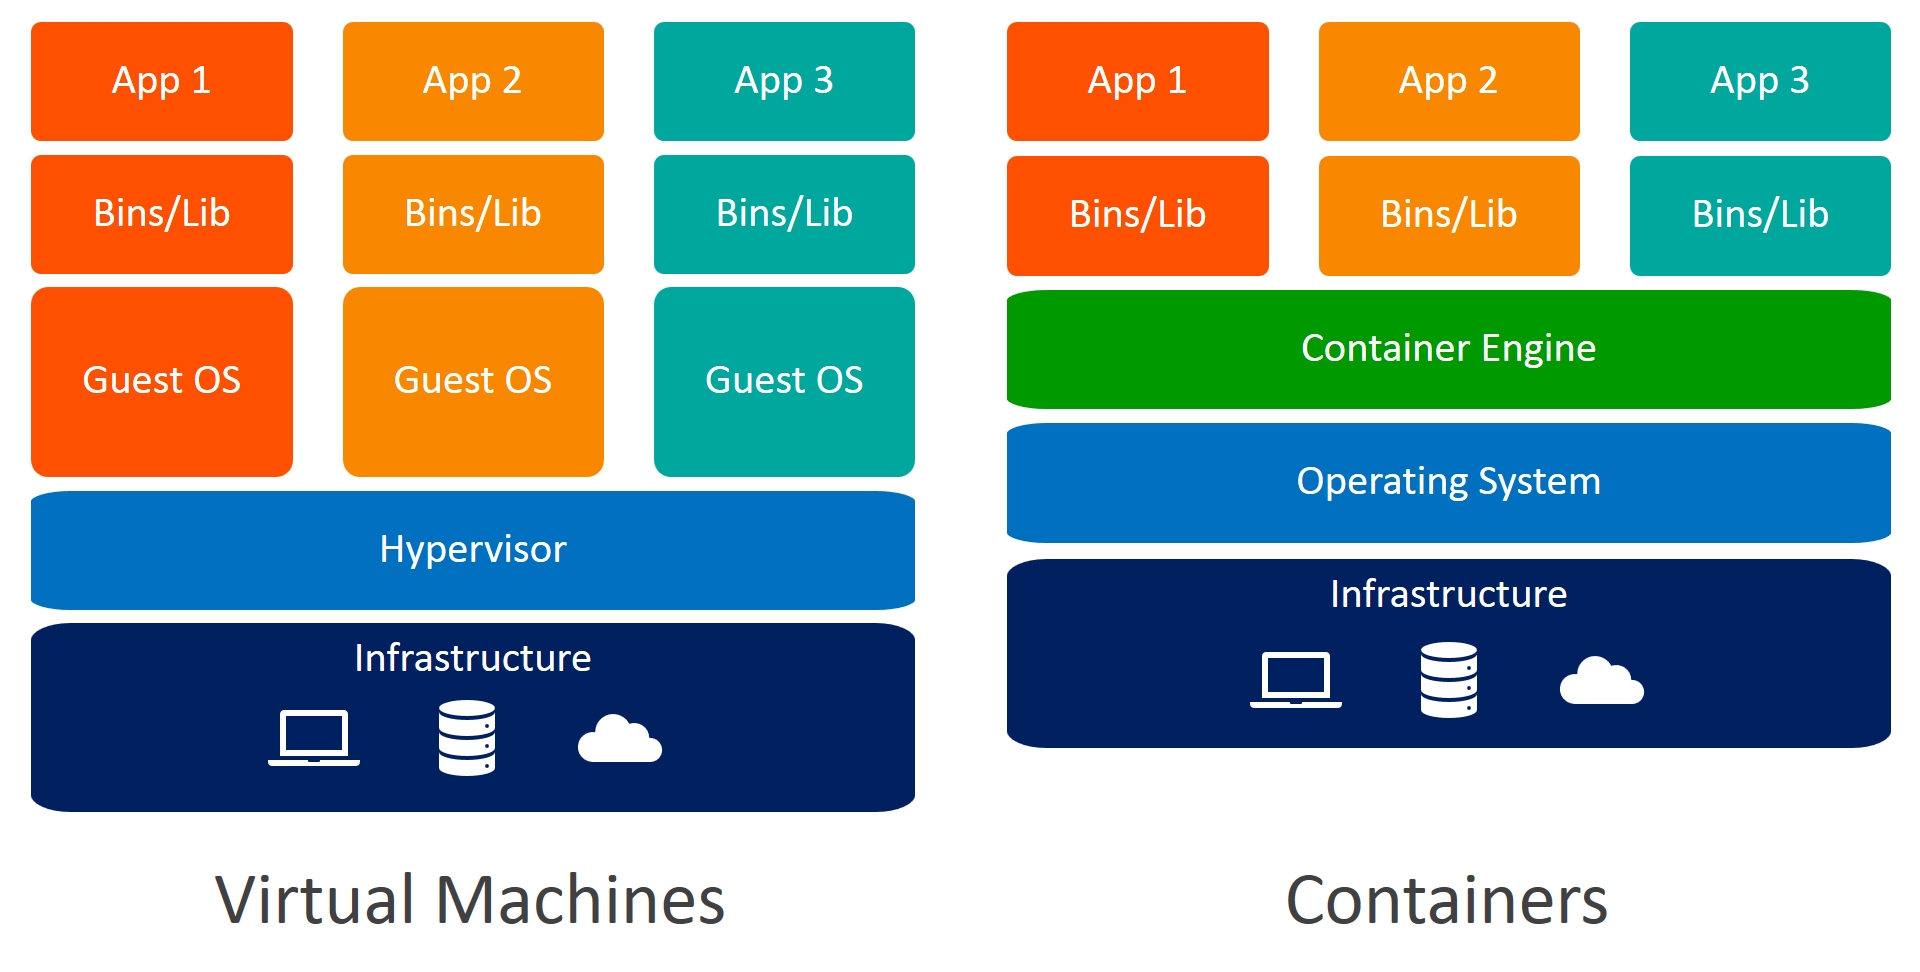
\includegraphics[width=1\linewidth]{figures/containervsvirtual}
    \caption{Porovnanie infraštruktúry kontajnera a virtualizácie \cite{containervsvirtual}}
	\label{kontaj}
\end{figure}

\subsection{Systémový a aplikačný kontajner}

Aplikačné kontajnery, ako napríklad Docker, zapuzdrujú súbory a knižnice aplikácie, ktoré sa majú spustiť na operačnom systéme. Aplikačné kontajnery umožňujú používateľovi vytvoriť a spustiť samostatný kontajner pre viacero nezávislých aplikácií alebo viacero služieb, ktoré tvoria jednu aplikáciu. Napríklad aplikačný kontajner by bol vhodný pre aplikáciu mikroslužieb, kde každá služba, ktorá tvorí aplikáciu, beží nezávisle jedna od druhej \cite{systemvsapli1}.

Systémové kontajnery, sú technologicky podobné kontajnerom aplikácií aj virtuálnym strojom. Systémový kontajner môže spúšťať operačný systém, podobne ako by operačný systém bežal zapuzdrený na virtuálnom stroji. Systémové kontajnery však neemulujú hardvér systému, namiesto toho fungujú podobne ako aplikačné kontajnery a používateľ si môže nainštalovať rôzne knižnice, jazyky a systémové databázy \cite{systemvsapli}.

Takže všeobecne, keď je potrebné distribuovať aplikáciu ako komponenty, aplikačné kontajnery sú skvelá voľba. Ak je iba operačný systém, do ktorého je treba nainštalovať rôzne knižnice, jazyky, databázy atď. vhodnejšie sú systémové kontajnery.
